\documentclass[a4paper,10pt]{article}
\usepackage[utf8]{inputenc}
\usepackage{amsthm}
\usepackage{amsmath}
\usepackage{xcolor}
\usepackage{float}
\newtheorem{definition}{Definition}
\newtheorem{claim}{Claim}
\newtheorem{theorem}{Theorem}
\newtheorem{example}{Example}
\newtheorem{condition}{Condition}
\newtheorem{proposition}{Proposition}
\usepackage{graphicx}
\definecolor{mygreen}{RGB}{0,150,0}
\newtheorem{lemma}{Lemma}
\usepackage{color}
\usepackage{calrsfs}
\usepackage{latexsym}
\usepackage{listings}
\usepackage{chngcntr}

\usepackage{mathrsfs}
\usepackage[colorlinks=true]{hyperref}
\hypersetup{
    colorlinks,
    citecolor=black,
    filecolor=black,
    linkcolor=blue,
    urlcolor=blue
}
\usepackage{ulem}
\def\st{\noindent}
\renewcommand\em{\it}
\renewcommand\emph{\textit}
\newcommand\red[1]{{\color{red}#1}}
\newcommand\blue[1]{{\color{blue}#1}}
\newcommand\green[1]{{\color{mygreen}#1}}
\newcommand\cancelr[1]{{\color{red}\sout{#1}}}
\newcommand\cancelg[1]{{\color{mygreen}\sout{#1}}}
%\newcommmand{\red}[1]{\textcolor{red}{#1}}
%\renewcommand\red[1]{{\color{red}#1}}
%opening
\title{L Plugin for Eclipse (Draft)}
\author{Evgenii Balai}
\def\no{{ not}\;}
\begin{document}

\maketitle
\st
\setcounter{tocdepth}{2}
\tableofcontents

\section{Installing the Plug-in}

\section{Using the Plug-in}
 
\subsection{Creating a New Project}
Every L program must be a part of a project. To create a project, go to the menu \texttt{File $\to$  New $\to$ Project} as shown in Figure \ref{fig1}.


\begin{figure}[H]
\centering
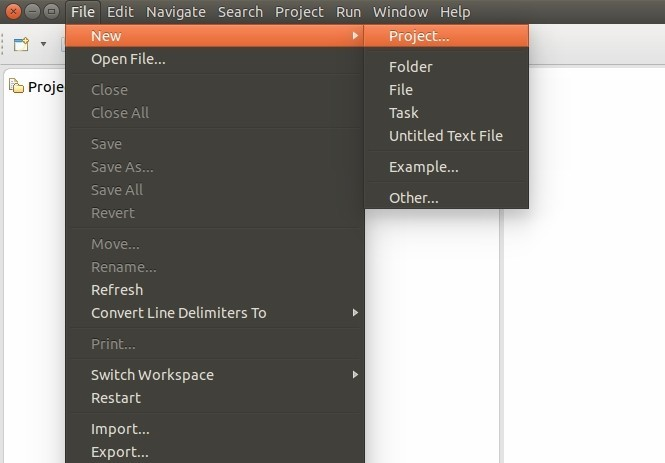
\includegraphics[width=0.6\textwidth]{1}
\caption{Creating a New Project (Menu)}\label{fig1}
\end{figure}
\noindent
In the opened window choose \texttt{General $\to$ Project} and click  \texttt{Next} as shown in Figure \ref{fig2}.
\begin{figure}[H]
\centering
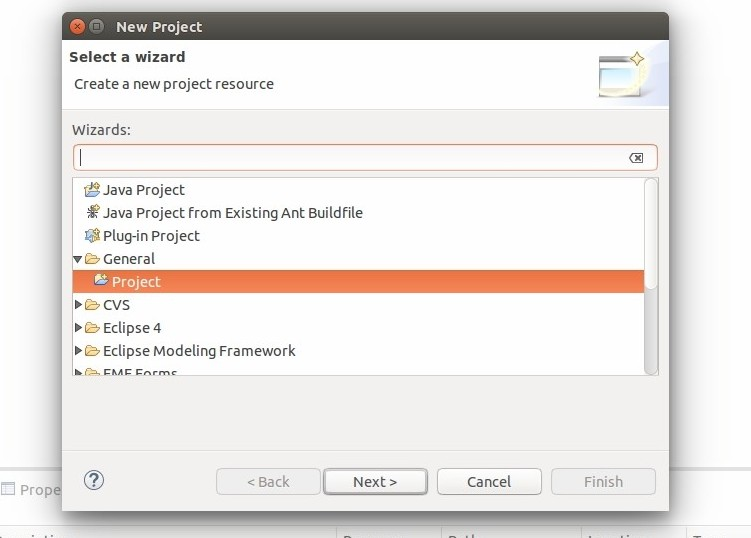
\includegraphics[width=0.8\textwidth]{2}
\caption{Choose the type of the project}\label{fig2}
\end{figure}


\noindent
In the next window shown on the screen type the name of the project (in our case the name is 
\texttt{safety\_ch5}) and click  \texttt{Finish}. See Figure \ref{fig3}.

\begin{figure}[h!]
\centering
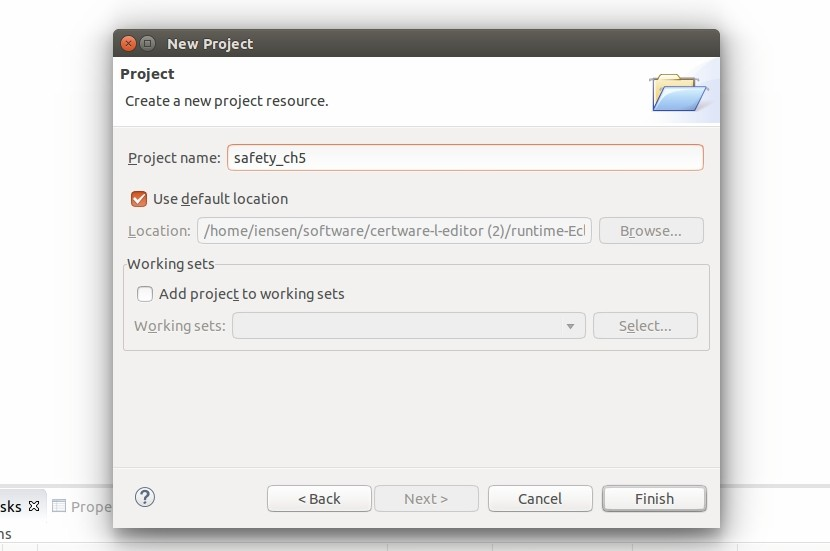
\includegraphics[width=0.8\textwidth]{3}
\caption{Final step of creating the project}\label{fig3}
\end{figure}

\noindent
You should see a new project is created and shown in the project explorer (a window in the top left corner), as in Figure \ref{fig4}.

\begin{figure}[h!]
\centering
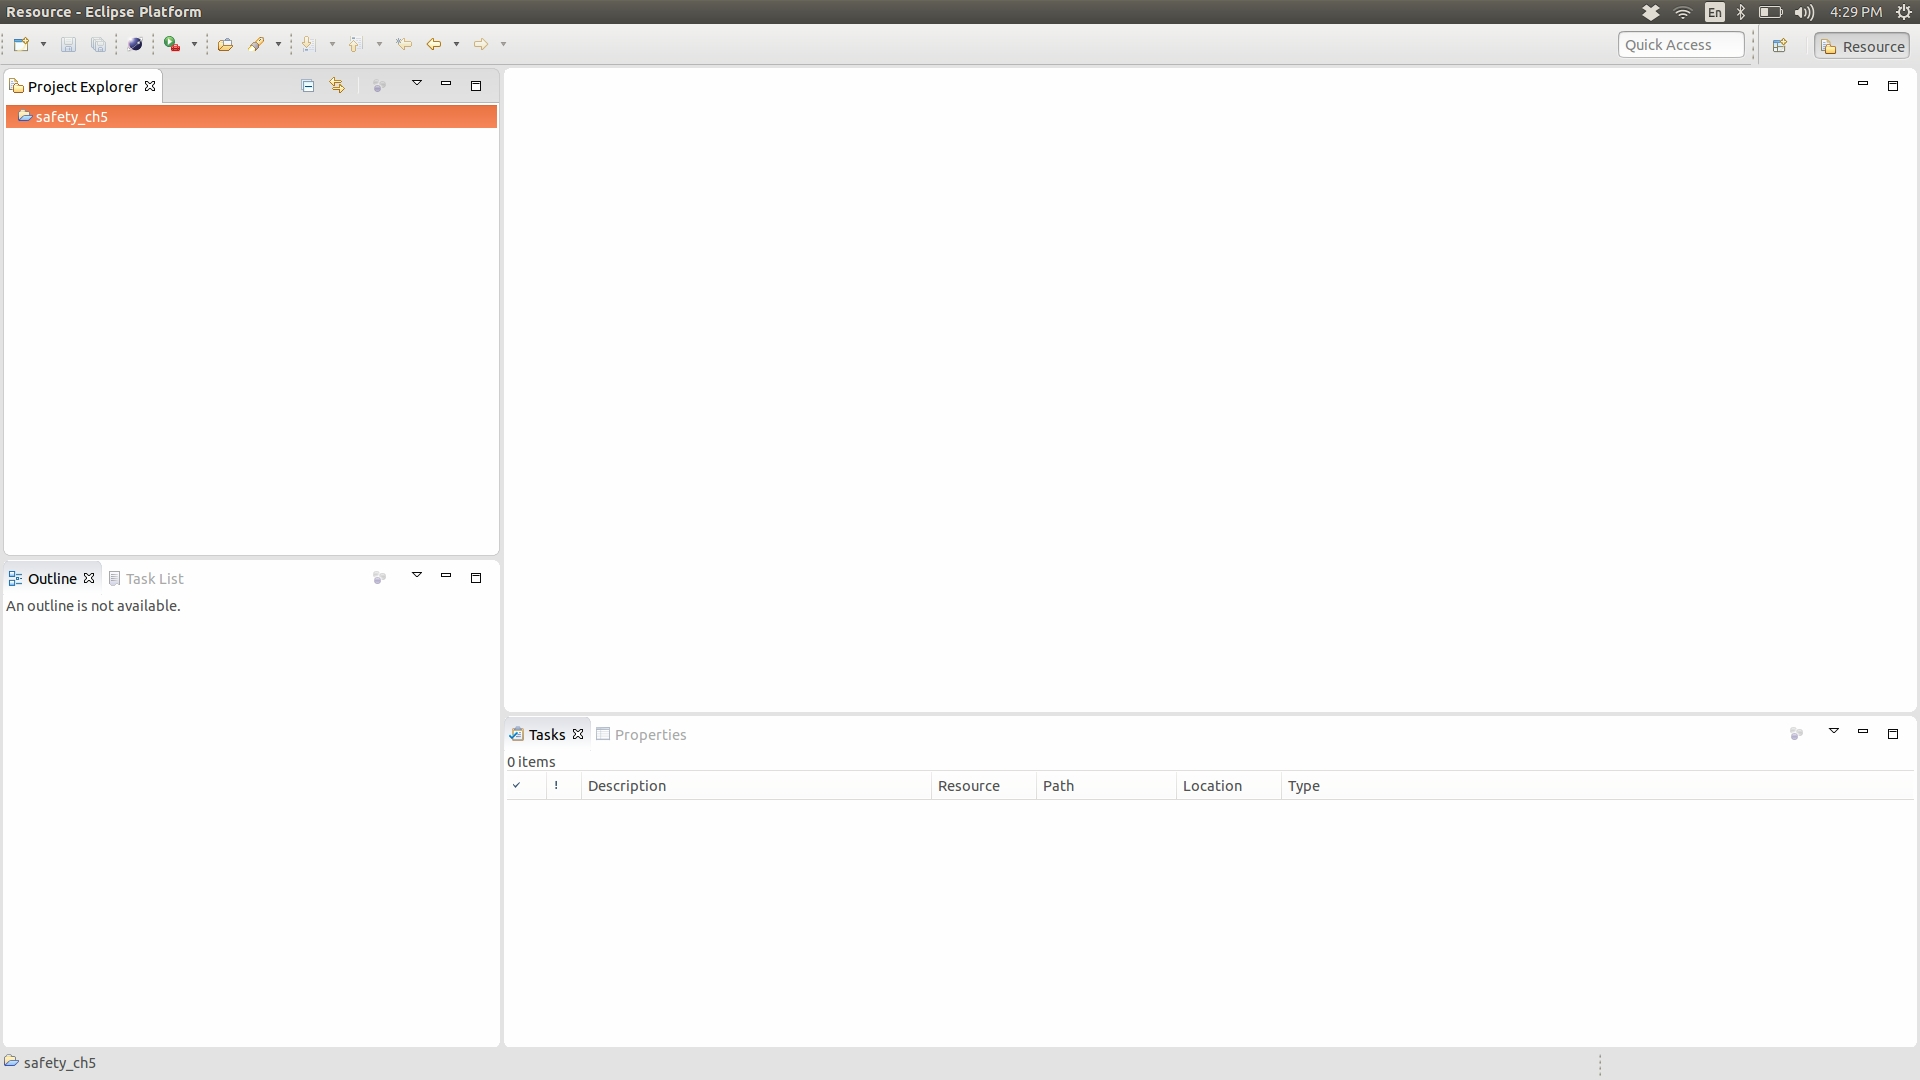
\includegraphics[width=1.0\textwidth]{4}
\caption{The newly created project is shown in the project explorer}\label{fig4}
\end{figure}






\subsection{Adding a New L Source File}

To create a file where an L program can be stored, right click  the project name in the project explorer and choose the menu \texttt{New $\to$ File} as shown in Figure \ref{fig5}.

\begin{figure}[h!]
\centering
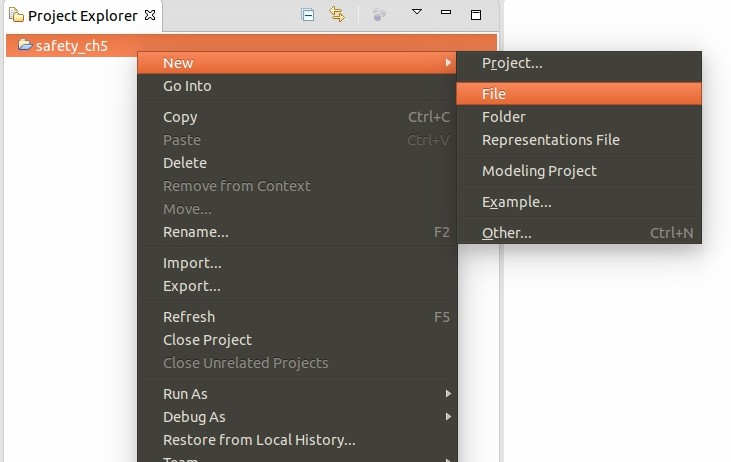
\includegraphics[width=1.0\textwidth]{5}
\caption{Creating a New L source file (Menu)}\label{fig5}
\end{figure}

\noindent
In the newly opened window type the name of the new file. \textbf{The name must have \texttt{.L} or \texttt{.l} suffix}. After the name is chosen, click  \texttt{Finish}. See Figure \ref{fig6}.

\begin{figure}[h!]
\centering
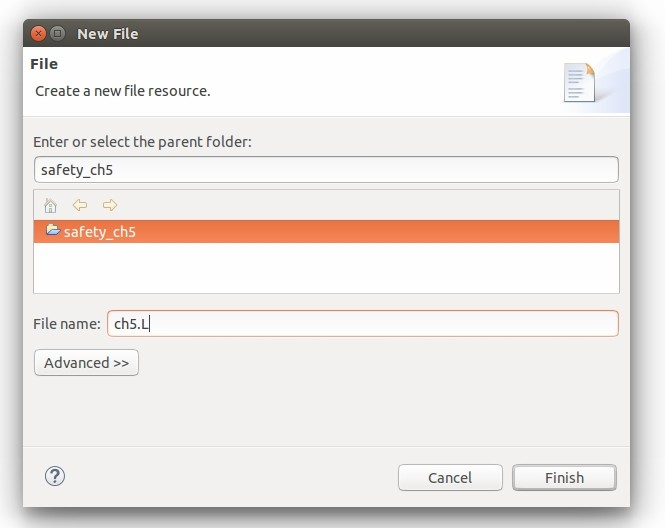
\includegraphics[width=0.8\textwidth]{6}
\caption{Giving the new file a name}\label{fig6}
\end{figure}

\noindent
If this is the first L source file added to the project, you should see a dialog shown in Figure \ref{fig7}.
 

\begin{figure}[h!]
\centering
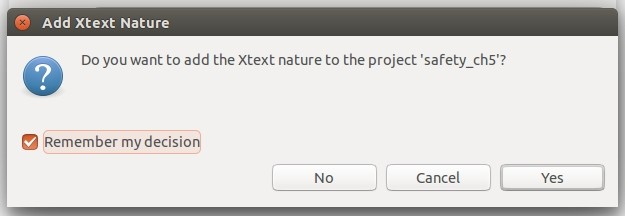
\includegraphics[width=0.8\textwidth]{7}
\caption{Adding Xtext nature to the project}\label{fig7}
\end{figure}

\noindent
Choose the option \texttt{Remember my decision} and click \texttt{Yes}.
After this step you should see the new file added to the project (and shown in the project explorer) 
and the L editor opened, as shown in Figure \ref{fig8}.
\subsection{Editing the File}

To edit the newly created file, switch the cursor to the largest text area of the workbench and start typing. See Figure \ref{fig8}.
\begin{figure}[h!]
\centering
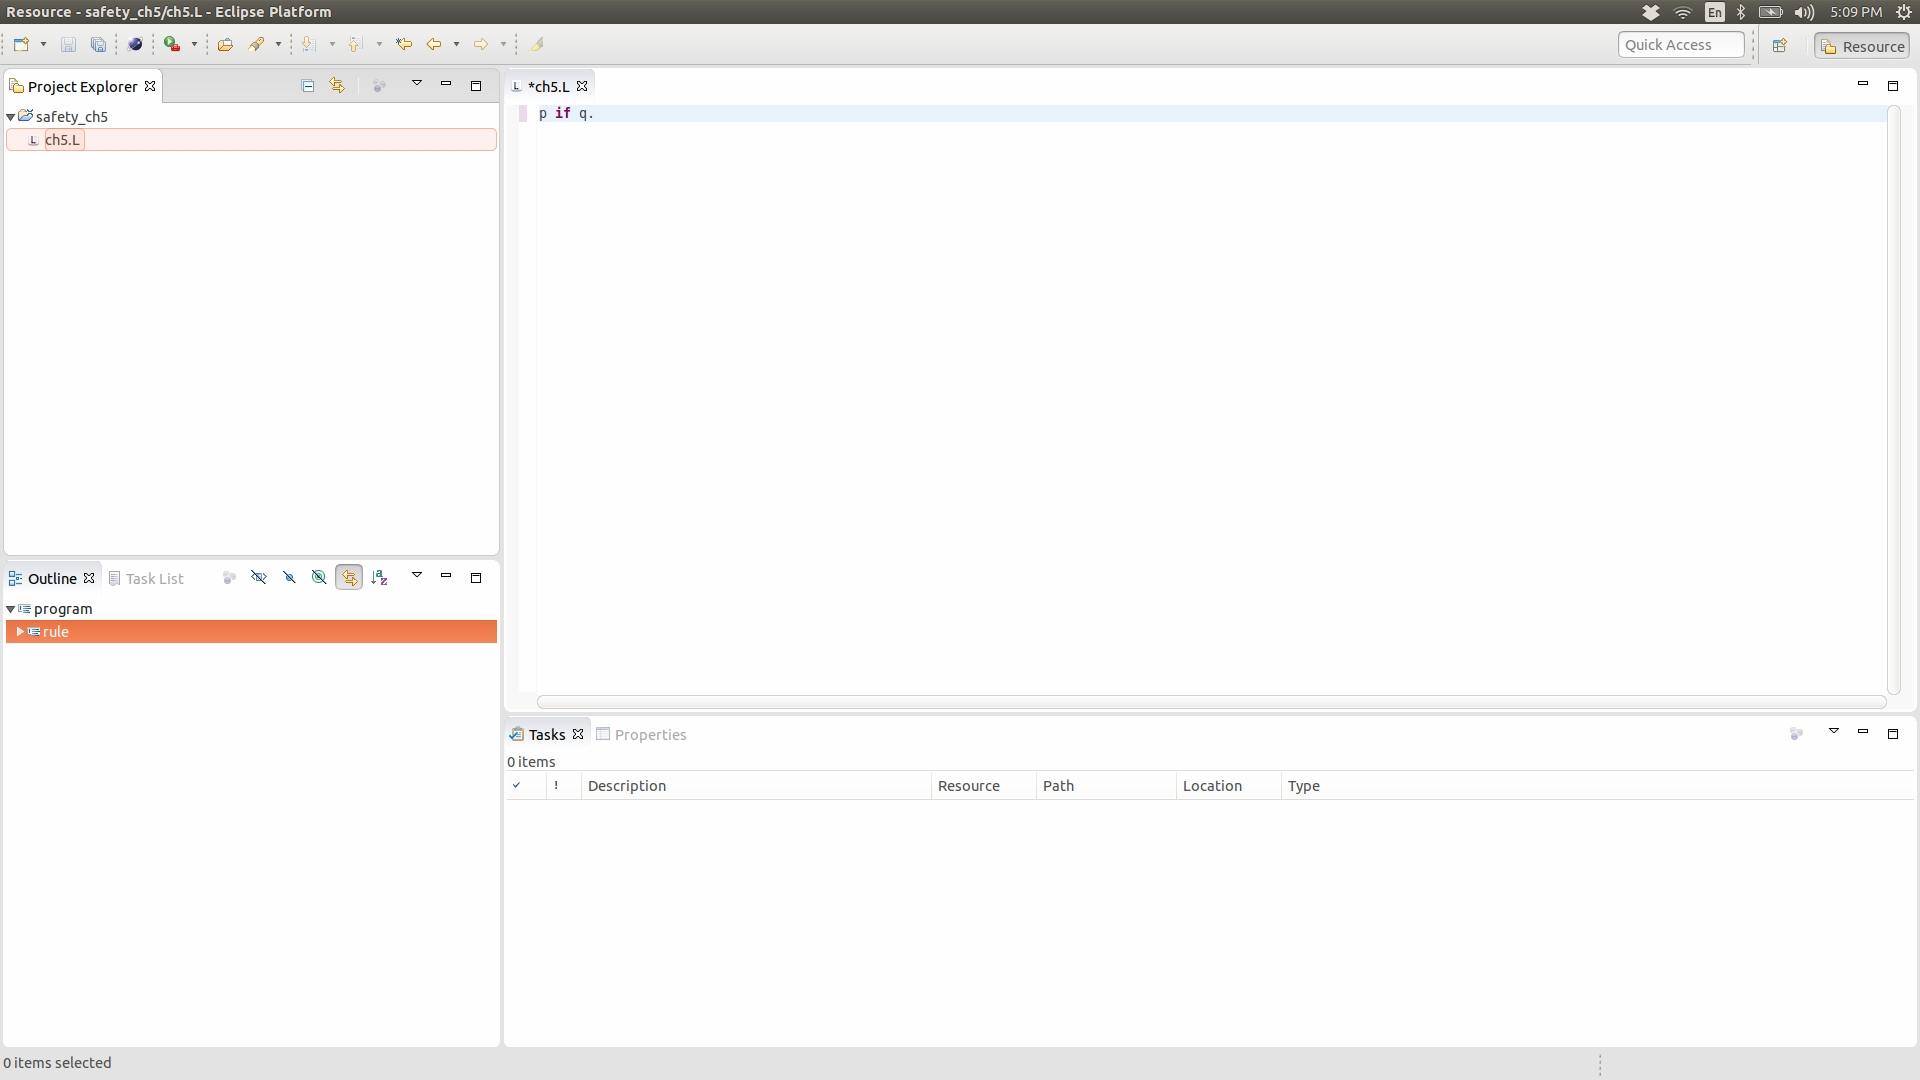
\includegraphics[width=1.0\textwidth]{8}
\caption{Editing the program}\label{fig8}
\end{figure}
The outline window in the bottom left corner shows the structure of the program.
If the program in the editor window has syntax errors, they will be shown in the bottom horizontal text area called \texttt{Problems}, as shown in Figure \ref{fig9}.


\begin{figure}[H]
\centering
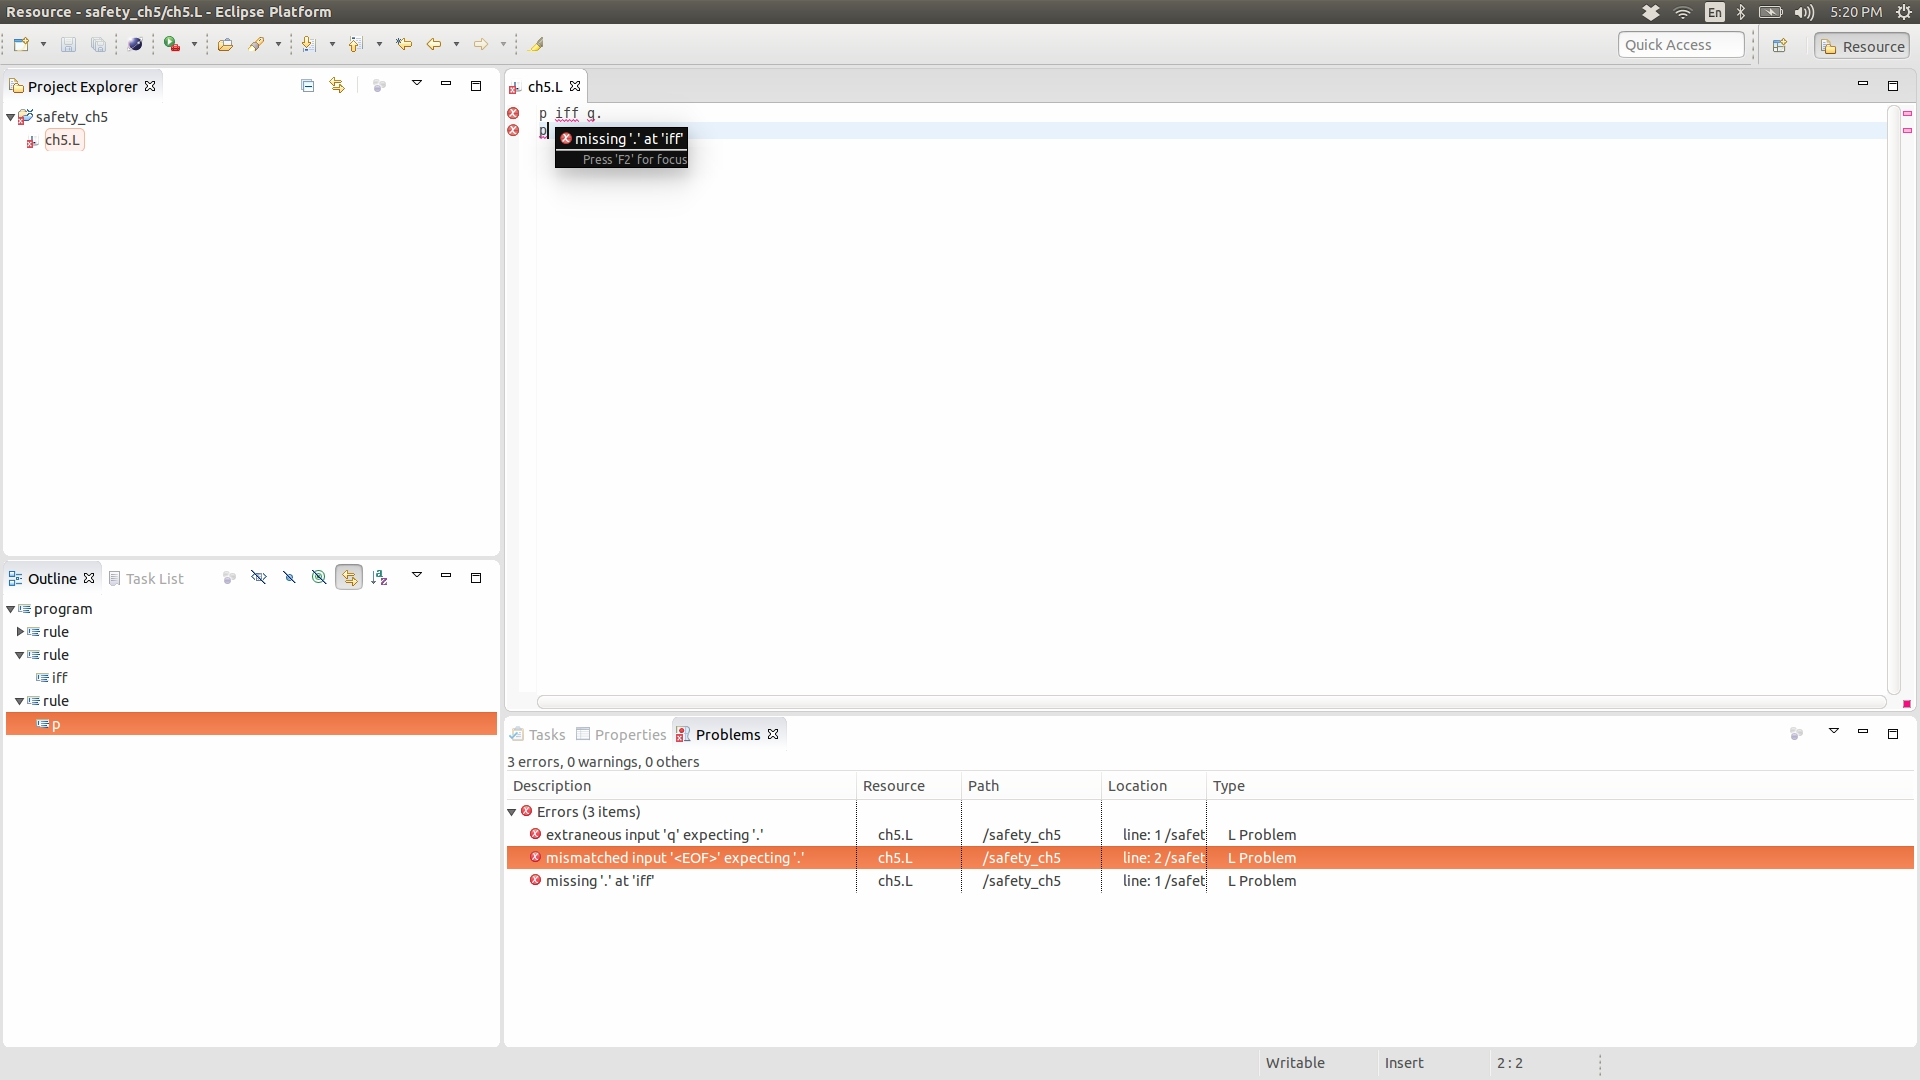
\includegraphics[width=1.0\textwidth]{9}
\caption{Erroneous program}\label{fig9}
\end{figure}


\noindent
The corresponding parts of the program will be underlined with red color in the editor. (If the window \texttt{Problems} is not shown, go to the menu \texttt{Window $\to$ Show View } and choose \texttt{Problems}.)
 
\subsection{Computing the Models of a Program}

To compute the models of the program stored in the L source file opened by the editor,
save the program (use \texttt{File $\to$ Save} menu or \texttt{Ctrl + S} shortcut) and  right click the editor window and click  the menu item \texttt{Compute Models}, as shown in Figure \ref{fig10}.


\begin{figure}[H]
\centering
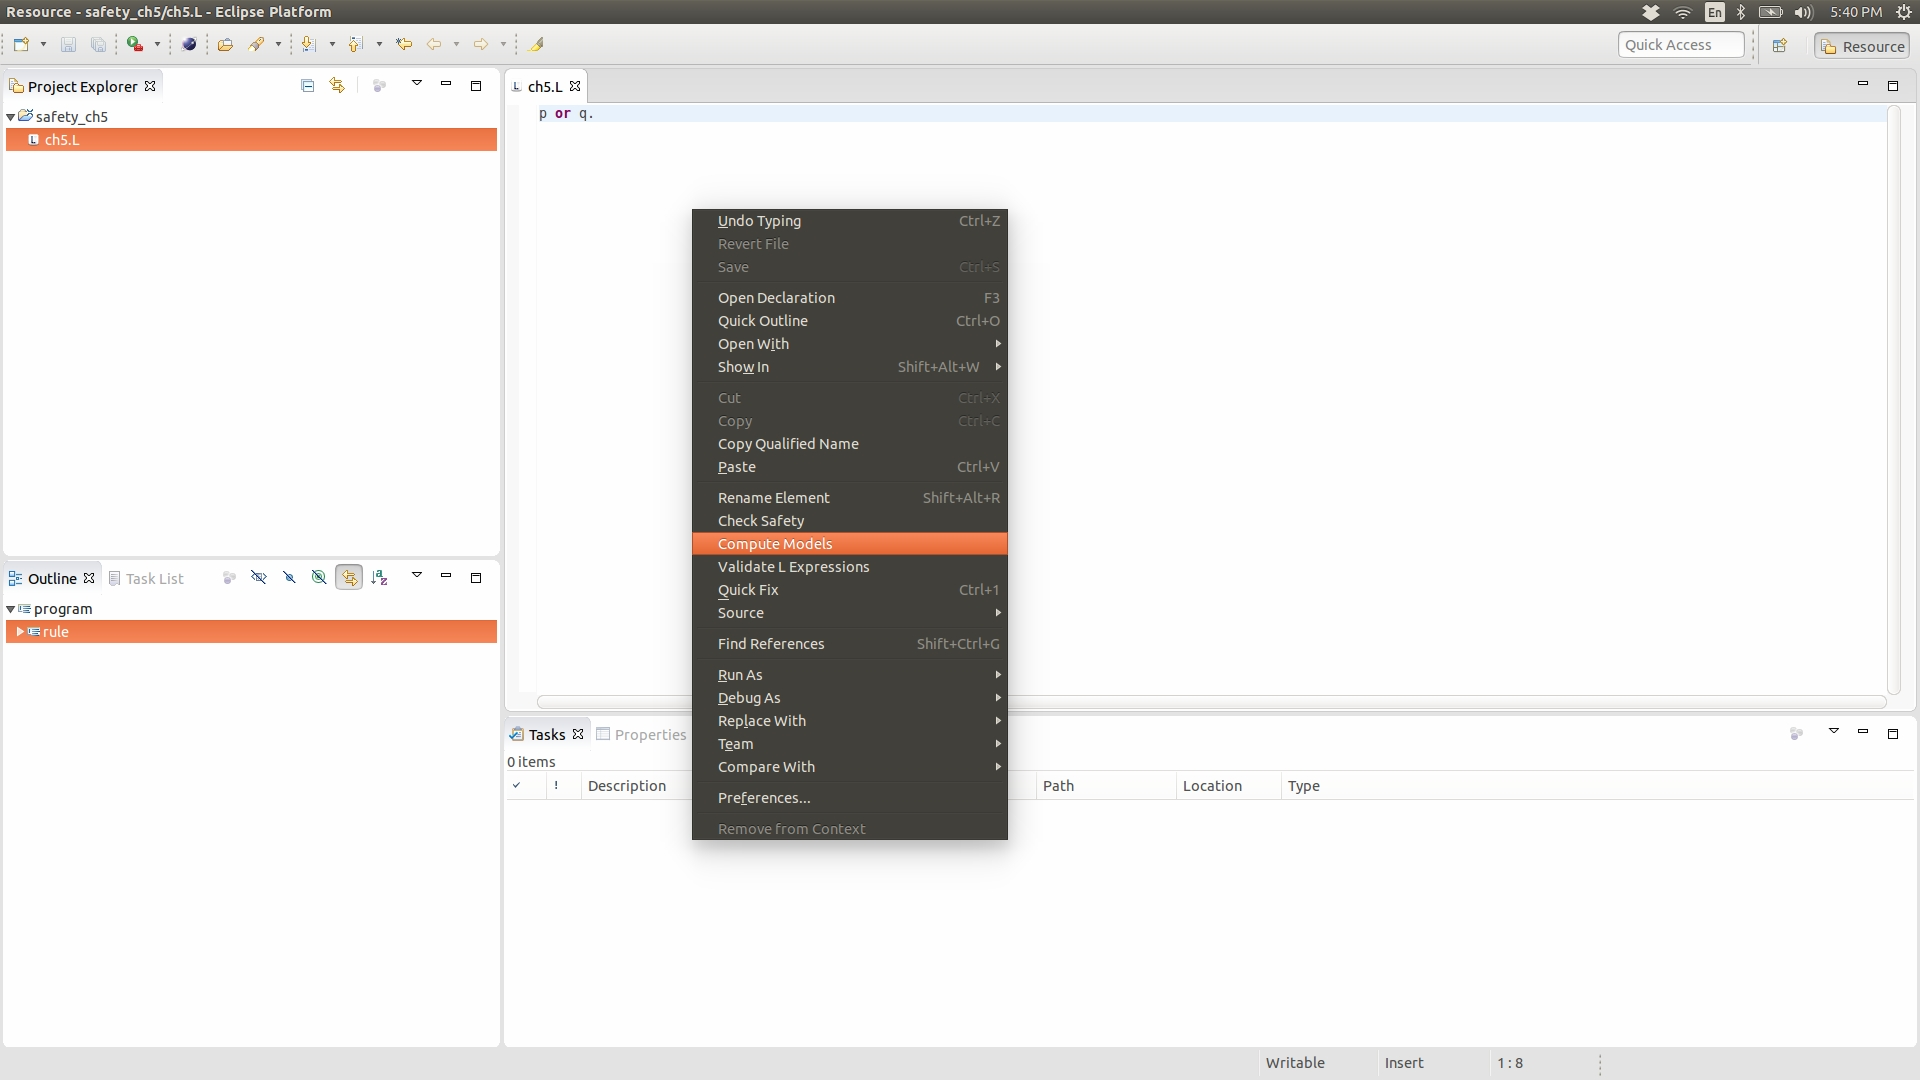
\includegraphics[width=1.0\textwidth]{10}
\caption{Computing the models of a program (Menu)}\label{fig10}
\end{figure}

The program shown in the editor in Figure 10 has two models, $p$ and $q$. After   \texttt{Compute Models} is clicked, the models will be shown in a separate editor, one per line, as shown in Figure \ref{fig11}.


\begin{figure}[H]
\centering
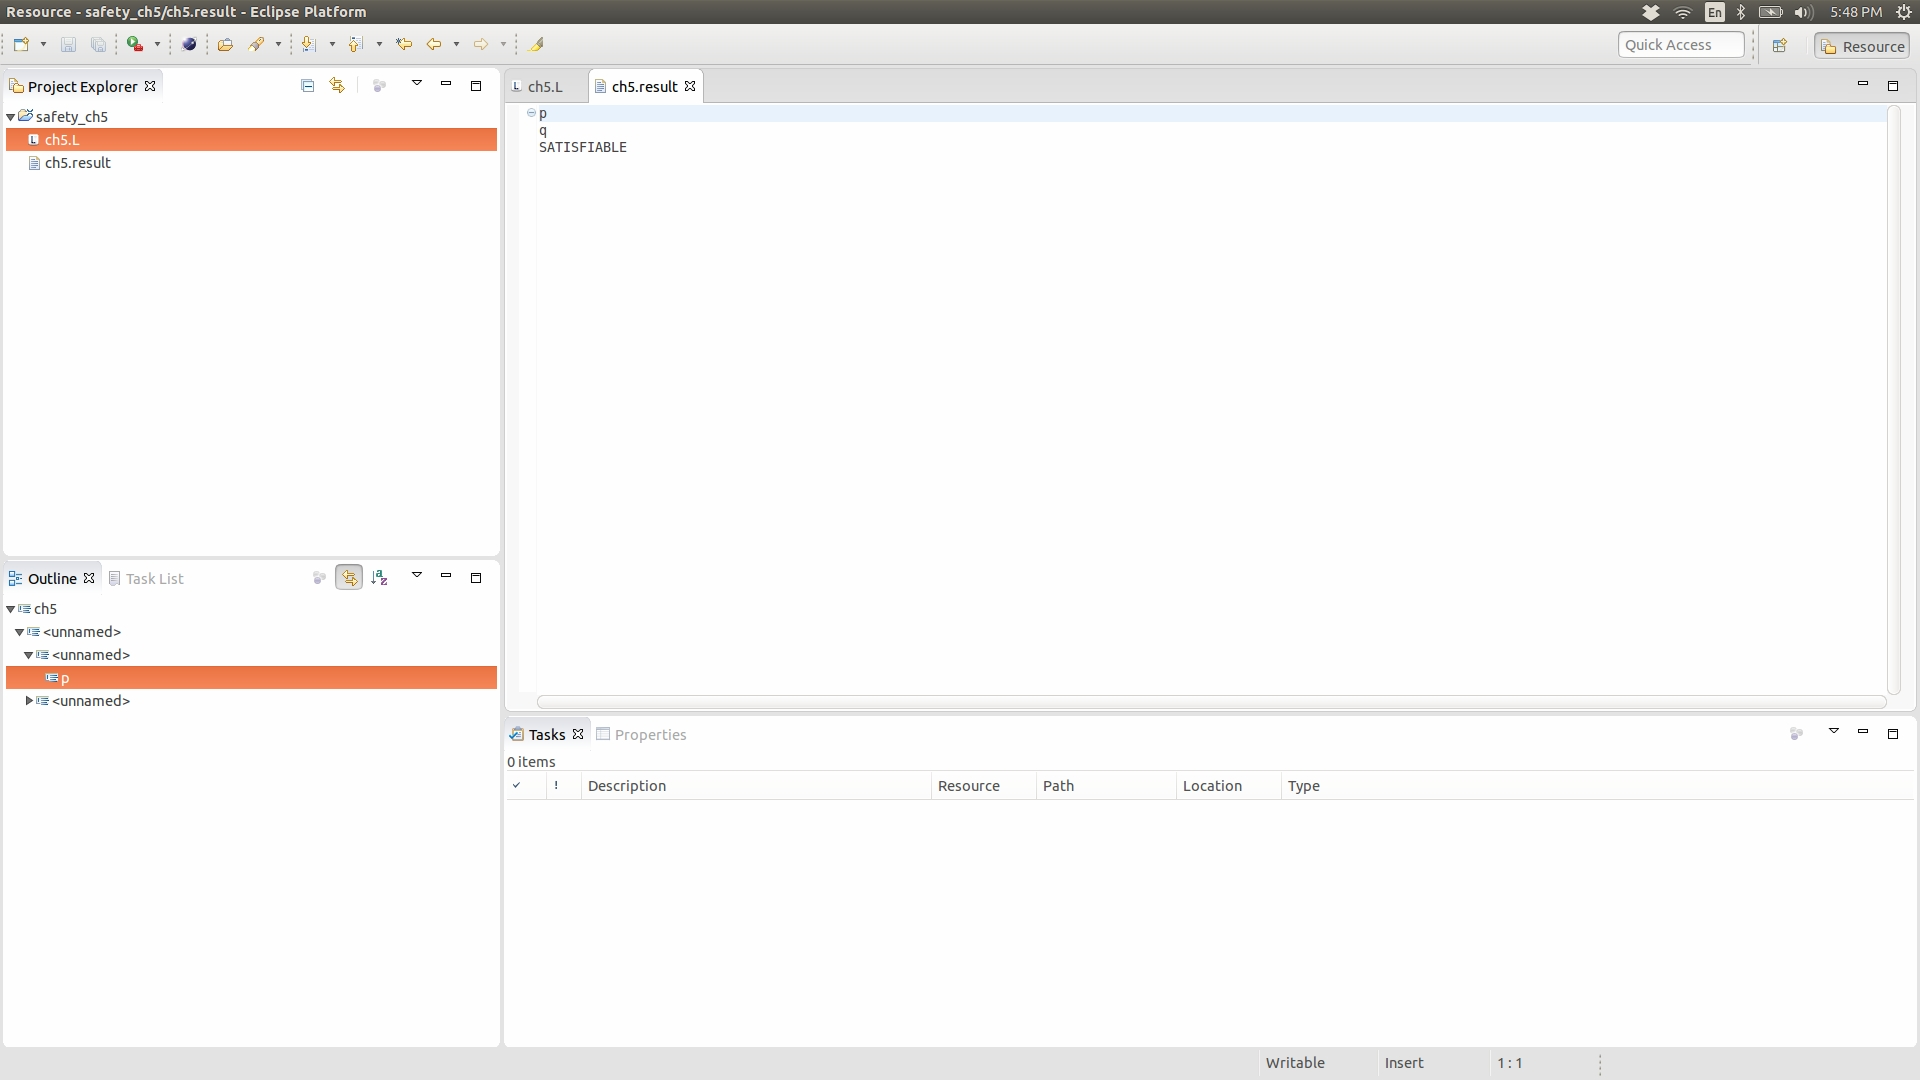
\includegraphics[width=1.0\textwidth]{11}
\caption{Computing the models of a program (Models)}\label{fig11}
\end{figure}



\subsection{Checking if Safety Requirements Defined by the Program are Met}  

To check if the safety requirements defined the by the program are met, load the program into the editor, switch the cursor to it and right click to show the context menu from Figure 10. Click  the menu item called \texttt{Check Safety}.
\begin{itemize}
\item if every model of the program includes the atom $safety\_reqts\_fully\_realised$, 
we say that \textit{safety requirements defined by the program are met};
\item otherwise, \textit{safety requirements defined by the program are not met.}
\end{itemize}

\noindent
For instance, the safety requirements defined by the program from \url{https://github.com/iensen/LtoASPtranslator/blob/master/src/examples/ch5.l}\\ which is based on chapter 5 of the EUR RVSM Safety Case \cite{?} are met. Therefore, if the program is entered into the editor and the menu item \texttt{Check Safety} is called, the  message shown in Figure \ref{fig12} indicating that the safety requirements are met can be observed.



\begin{figure}[H]
\centering
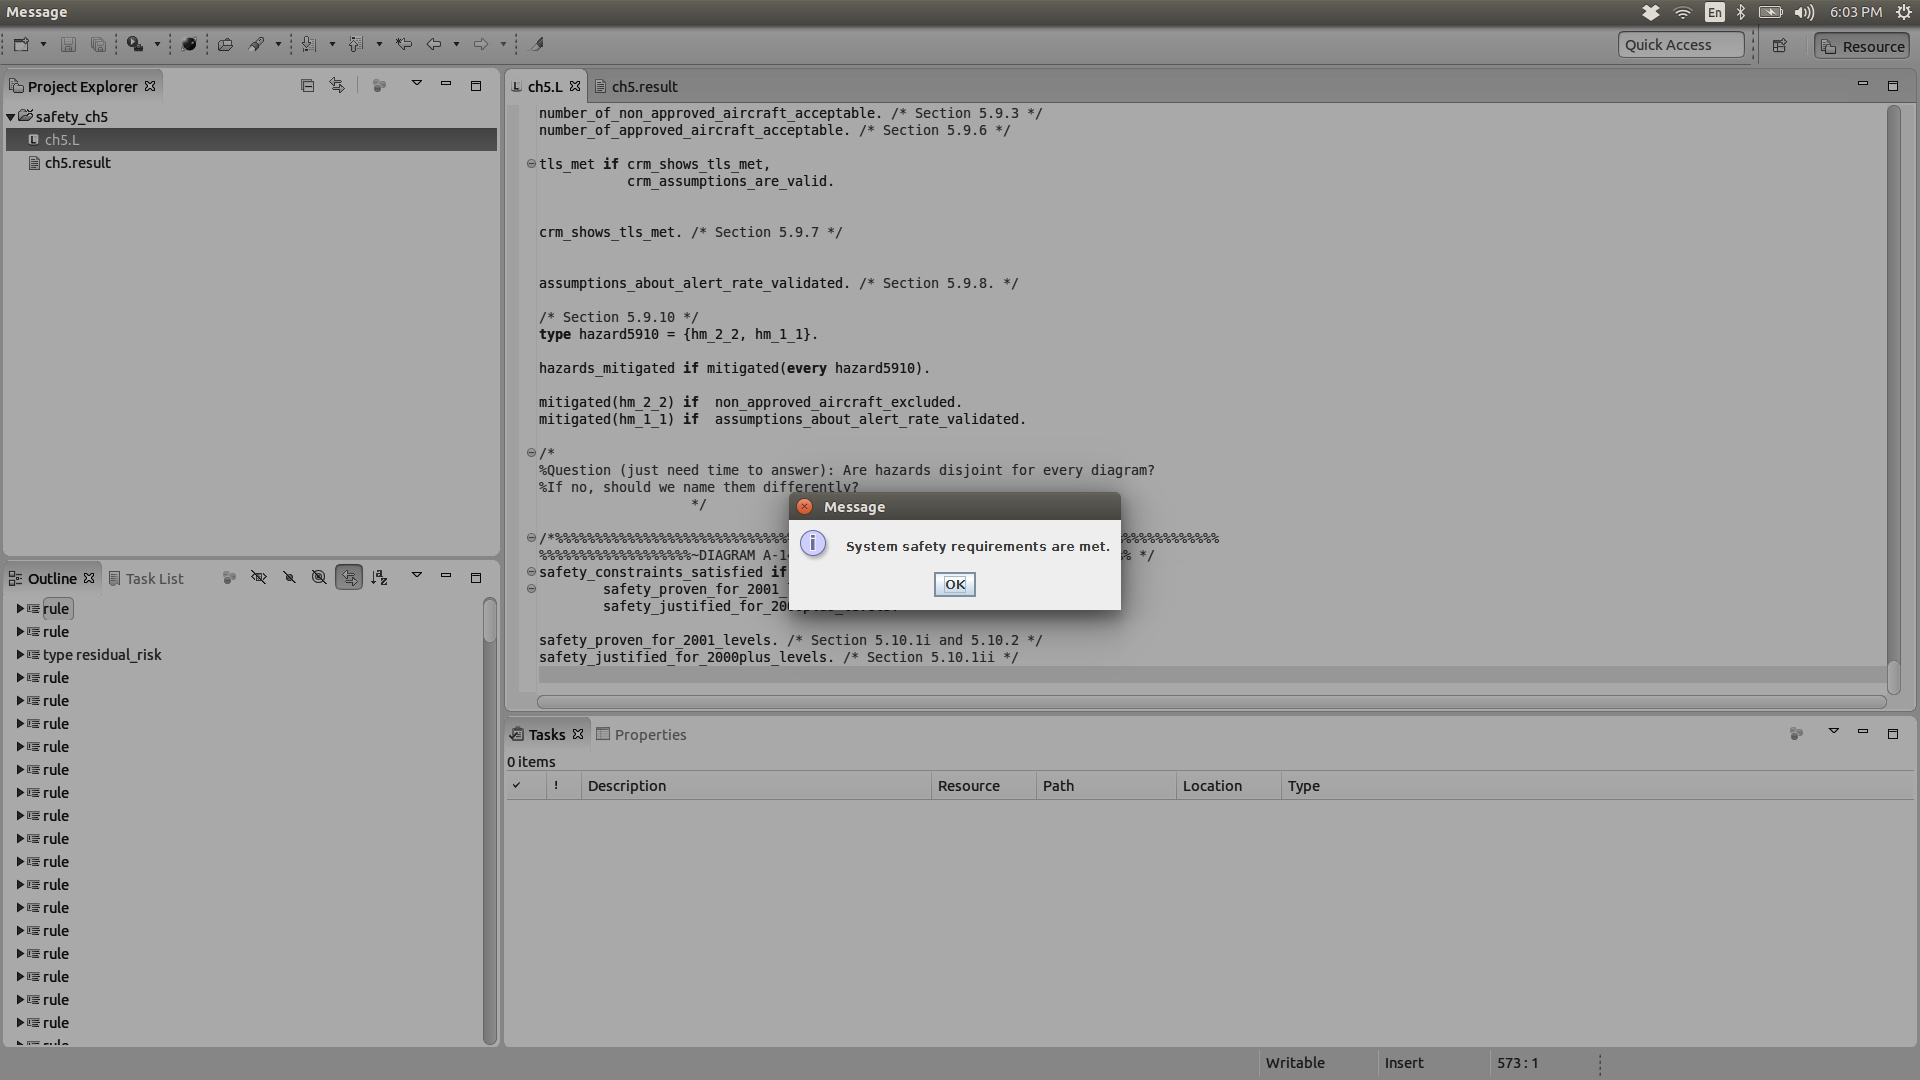
\includegraphics[width=0.85\textwidth]{12}
\caption{Checking safety - 1}\label{fig12}
\end{figure}

\noindent
However, if, for example, the fact \texttt{mitigated(level\_busts)} (indicating that level busts threat was mitigated) is removed, the safety requirements defined by the program are no longer met. The corresponding message is shown in Figure \ref{fig13}.

 
\begin{figure}[H]
\centering
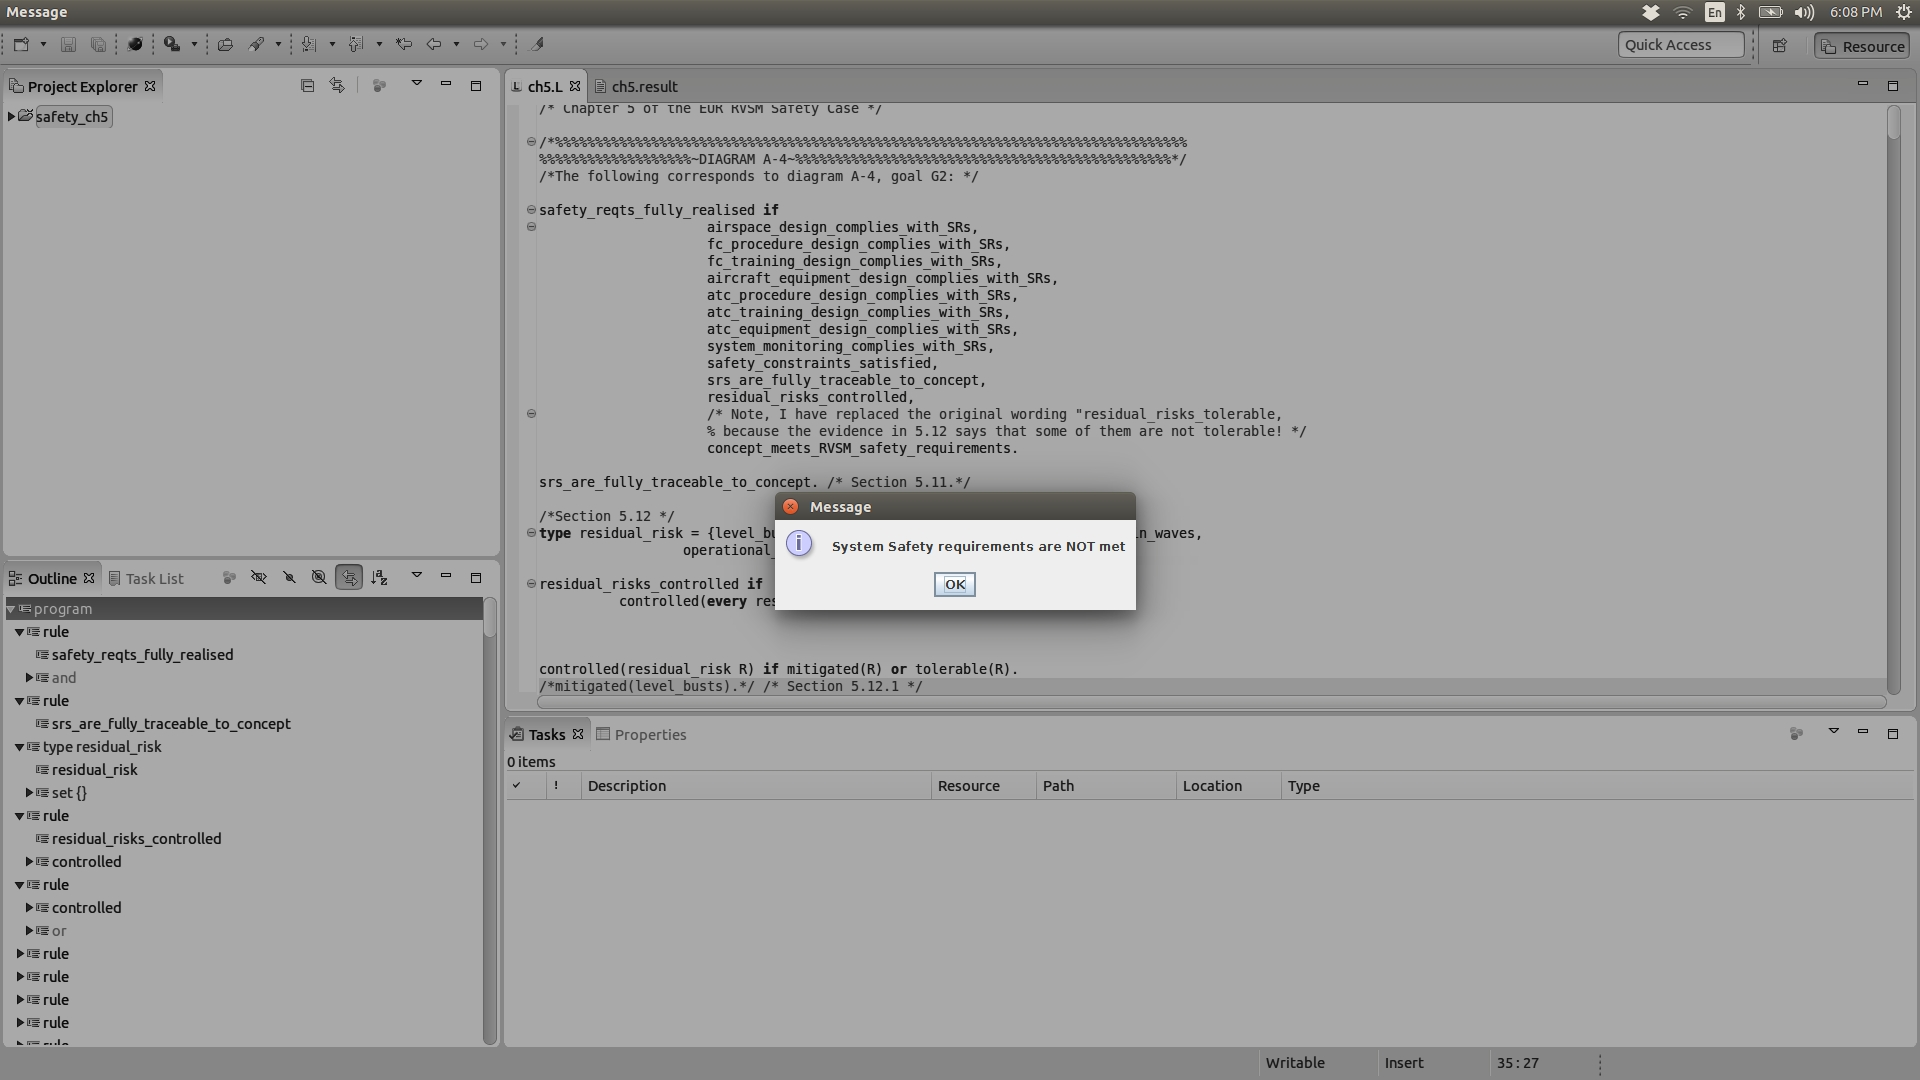
\includegraphics[width=0.85\textwidth]{13}
\caption{Checking safety - 2}\label{fig13}
\end{figure}



\end{document}


%%% Local Variables:
%%% mode: latex
%%% TeX-master: t
%%% End:
